\section{Implementación del prototipo}\label{section:prototype}

El prototipo implementado se concibe como una aplicación web. Se compone de cuatro componentes: crawler, catálogo de datos, generador de consultas 
e interfaz de usuario; los cuales se corresponden con la concepción y el diseño del sistema propuesto en el capítulo \ref{chapter:proposal}, 
ilustrado en la figura \ref{fig:arquitectura}. 
La lógica de los análisis sintáctico y léxico del lenguaje de dominio específico, DSL, propuesto fue incluida como parte 
del generador de consultas. 

Por cuestiones de tiempo no se pudo concretar una implementación del generador de pipelines. 
La implementación de este componente plantea desafíos considerables. Primeramente, 
este debe ser independiente de los sistemas gestores de bases de datos de la fuente y del almacén de datos. 
Además, su implementación implica la implementación de la lógica para los tipos de extracción y carga de datos. 
Por otro lado, el generador de pipelines también es el encargado de ejecutar los pipelines de forma autónoma, 
por tanto se debe implementar un mecanismo de captura de eventos que dictamine en que momento ejecutar el pipeline.

Durante el proceso de investigación previo a la implementación se identificó que con la utilización de la  
plataforma Apache Airflow\footnote{https://airflow.apache.org} se pueden satisfacer varios de los 
requisitos funcionales del generador de pipelines. Airflow es una herramienta de orquestación de flujos de 
trabajo de procesamiento de datos que permite a los desarrolladores definir y monitorear flujos de trabajo. 
Un flujo de trabajo es modelado como un grafo dirigido y ac\'iclico, (DAG), cuyos nodos representan tareas y los 
arcos modelan la dependencia entre las tareas. Los DAG son definidos mediante scripts de Python, en los cuales 
se especifican las tareas a realizar mediante operadores de Airflow y su \'orden. Luego, generar un DAG 
cuyas tareas sean la ejecución de las consultas construidas por el generador de consultas para la población de 
un escenario analítico determinado implica generar 
din\'amicamente un script de Python que de definición al DAG. Además, la estructura de dicho script 
no es estática pues el n\'umero de tareas a realizar y su orden dependen del escenario analítico a poblar,
y los operadores de Airflow para la ejecución de las consultas varían según el sistema gestor de base de 
datos de la fuente y del sistema destino. Por tanto, la generación dinámica del script de python que define un DAG 
no es un proceso trivial.

Luego, la implementación del generador de pipelines mediante el uso de Airflow plantea desafíos significativos que 
no pudieron ser resueltos debido al alto volumen de trabajo necesario para implementar otros componentes del marco 
de trabajo propuesto y al tiempo disponible para la realización de esta investigación. Por lo tanto, se propone 
la implementación del generador de pipelines como trabajo futuro.

\subsection{Organización de los archivos}

La lógica de cada uno de los componentes de la aplicación se encuentra separada por carpetas. Cada componente 
posee su propia carpeta identificada con el nombre del componente en inglés, a excepción de la interfaz de usuario 
cuya carpeta es nombrada \textbf{pages} y su script principal se encuentra en la raíz del proyecto con el nombre de 
\textbf{MainPage.py}. Todos los datos derivados de la ejecución de la lógica de cada uno de los componentes 
se almacena dentro de la carpeta \textbf{data}. La carpeta \textbf{utils} guarda scripts de algoritmos usados 
en varias partes de la aplicación, concretamente posee scripts con algoritmos para la carga y escritura de los 
grafos y \'arboles de join en el disco.

\subsection{Fuentes de datos}

El prototipo maneja una única fuente de datos a la vez, aunque es posible considerar varias 
fuentes de datos para un mismo almacén de datos de destino. Para esto se debe definir un script del DSL por 
cada fuente de datos que alimente el almacén de datos. Las primeras consultas de creación generadas que se ejecuten 
para dicho almacén determinarán el nombre de las tablas de las dimensiones y de los hechos, as\'i como 
como el nombre de sus atributos, sus tipos y restricciones. Luego, para alimentar el almacén de datos con otras 
fuentes, basta con ejecutar las consultas de selección generadas a partir del script correspondiente a 
dicha fuente y, con posterioridad, insertar en el almacén los valores extra\'idos.

\subsection{Crawler}

El Crawler constituye un elemento de interdependencia dentro del prototipo en relación con los sistemas 
que administran las fuentes de datos, específicamente con los los sistemas de gestión de bases de datos, (SGBD). 
Con el objetivo de lograr una 
mayor extensibilidad, se plantea la creación de una clase abstracta llamada \textbf{crawler}, la cual establecerá 
el comportamiento general de este componente. De este modo, se delega a las implementaciones específicas para cada 
SGBD la definición de la forma en que se llevan a cabo las operaciones, como se muestra en la figura \ref{fig:crawler}. 
El ejemplo de código \ref{code:crawler} muestra la definición de la clase abstracta \textbf{crawler}.

\begin{figure}[H]
    \centering
    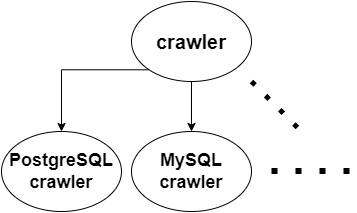
\includegraphics[width=0.5\textwidth]{Graphics/crawler_class.drawio.png}
    \caption{Jerarquía de la clase abstracta crawler}
    \label{fig:crawler}
\end{figure}

\begin{lstlisting}[label={code:crawler}, caption={Definición de la clase abstracta crawler}, language={python}]
    import abc

    class Crawler(metaclass=abc.ABCMeta):
        def __init__(self, dbname, user, password, host, port) -> None:
            self.dbname = dbname
            self.user = user
            self.password = password
            self.host = host
            self.port = port
            self._db_params = {'dbname': dbname, 'user': user, 'password': password, 'host': host, 'port': port}
            self._metadata_str = ''
            self._db_dict = {}

        @abc.abstractmethod
        def explore_db(self):
            pass
        
        @abc.abstractmethod
        def export_metadata_to_file(self):
            pass

\end{lstlisting}

La implementación de esta clase se encuentra en el archivo \textbf{crawler.py} de la carpeta del componente homónimo. Los 
campos de la clase se corresponden con la información necesaria para establecer una conexión con una base de 
datos. 

El método \textbf{explore\_db} se encarga de recopilar los metadatos de la fuente de datos con nombre \textbf{dbname}. 
Los metadatos recopilados son, como ya se mencion\'o en el cap\'itulo de concepción y diseño, los nombres de las 
tablas de la base de datos fuente, por cada tabla se obtienen sus
atributos, por cada atributo su tipo y si son llaves primarias. Además, por cada tabla
se obtienen los atributos que son llaves foráneas y, por cada una, se extrae el nombre
de la tabla a la que referencian y el atributo referenciado. Los metadatos recopilados se almacenan en el diccionario 
\textbf{\_db\_dict}, el cual tiene como llaves los nombres de las tablas de la base 
de datos y como valores otros diccionarios que poseen dos llaves: \textbf{attributes} y \textbf{relations}. 
El valor de \textbf{attributes} es una lista de tuplas de dos o tres elementos, una por cada atributo de la tabla. 
Las tuplas de dos elementos almacenan el nombre del atributo y el tipo, las de tres almacenan además un indicador 
que expresa si el atributo es llave primaria, for\'anea o ambas. El valor de \textbf{relations} es una lista de 
tuplas de tres elementos, una por cada atributo que es una llave foránea de la tabla. El primer elemento es el nombre 
de la llave for\'anea en la tabla, el segundo el nombre de la tabla referenciada y el tercero el atributo referenciado. 
El ejemplo de c\'odigo \ref{dbdict} muestra la estructura del diccionario \textbf{\_db\_dict}. 

\begin{lstlisting}[label={dbdict}, caption={Estructura del diccionario \textbf{\_db\_dict}}]
_db_dict: {
    'tabla_1' : {
        attributes: [(atr_1, tipo, PK FK), ..., (atr_n, type)]
        relations: [(atr_1, tabla_ref, atr_ref), ...]
    }
    .
    .
    .
    'tabla_n': { ... }
}
\end{lstlisting}

Además, el método \textbf{explore\_db} tiene la responsabilidad de llenar la cadena de texto \textbf{\_metadata\_str} 
que almacena los metadatos recopilados en un formato m\'as expresivo para luego ser mostrado al desarrollador.

El método \textbf{export\_metadata\_to\_file} se encarga de guardar \textbf{\_db\_dict} y \textbf{\_metadata\_str} en el disco, 
en la ruta \textbf{data/schemas}. La carpeta \textbf{schemas} contiene una carpeta por cada base de datos, identificada 
por el nombre de la base de datos, en la cual se almacena \textbf{\_db\_dict} en formato json y 
\textbf{\_metadata\_str} en formato txt.

En esta primera entrega del prototipo solo se implement\'o un crawler para PostgreSQL. Su l\'ogica 
se encuentra en el archivo \textbf{postgreSQL\_crawler.py}. Los metadatos son recopilados mediante consultas 
realizadas
a la tabla \textbf{information\_schema} de la base de datos fuente, utilizando para la ejecución de las consultas 
el adaptador de PostgreSQL para python \textbf{psycopg2}.




\subsection{Catálogo de Datos}

El catálogo de datos es un servidor de bases de datos de Neo4j que contiene un grafo por cada base de datos 
fuente que haya sido explorada por la aplicación. Cada vez que el crawler explora una base de datos fuente nueva se crea 
un grafo de base de datos de Neo4j para almacenar sus metadatos.

La comunicación de la aplicación con el Catálogo de Datos es mediada por la clase \textbf{DataCatalogHandler} 
presente en el script \textbf{handler.py} de la carpeta \textbf{data\_catalog}. En el ejemplo de c\'odigo 
\ref{code:catalog} se muestra parte del código de dicha clase.

\begin{lstlisting}[label={code:catalog}, caption={Clase DataCatalogHandler}, language={python}]
    class DataCatalogHandler():
        def __init__(self, db_dict, db_name, user, password, uri) -> None:
            self.db_dict = db_dict
            self._user = user
            self._password = password
            self._uri = uri
            self.db_name = db_name
            self.join_graph = None

        def create_database(self):
            # Omitted implementation

        def populate_graph_database(self):
            # Omitted implementation

        def export_join_graph(self):
            # Omitted implementation

\end{lstlisting}

El campo \textbf{db\_dict} hace referencia al diccionario de la base de datos confeccionado por el crawler, ver ejemplo de c\'odigo \ref{dbdict}, 
\textbf{db\_name} almacena el  
nombre de la base de datos fuente, \textbf{join\_graph} almacena una referencia en memoria del grafo de joins construido 
durante la ejecución de \textbf{export\_join\_graph}. El resto de atributos 
son los necesarios para establecer una conexión con una base de datos de Neo4j; en especial, el campo \textbf{\_uri} 
es una cadena de texto que contiene el protocolo de comunicación con el servidor de Neo4j, su ip y su puerto. 

El método \textbf{create\_database} crea una base de datos de Neo4j en el catálogo de datos dedicada a la 
fuente de datos con nombre \textbf{db\_name} y con diccionario de metadatos \textbf{db\_dict}. 

El método \textbf{populate\_graph\_database} se encarga de poblar la base de datos de Neo4j con los metadatos
recopilados. Se crea 
un nodo por cada llave 
de \textbf{db\_dict} con las propiedades \textbf{name} que almacena el nombre de la tabla, \textbf{pks} que es una 
lista con los nombres de los atributos que son llaves primarias y, por \'ultimo, \textbf{attributes} que 
es la lista de tuplas correspondiente a la llave attributes del diccionario que devuelve \textbf{db\_dict} como valor
al ser indexado  en el nombre de la tabla en cuestión (\textbf{db\_dict[table\_name]}). Además, se crea una relación direccionada por cada llave for\'anea 
presente en la lista correspondiente a la llave relations del diccionario que devuelve \textbf{db\_dict} 
como valor al ser indexado en el nombre de la tabla en cuestión. La dirección de la relación lo dictamina 
el sentido de la referencia de la llave 
for\'anea, tal y como se expuso en el capitulo \ref{chapter:proposal} en la sección referente al catálogo de 
datos.

El método \textbf{export\_join\_graph} es el encargado de construir, a partir de la base de datos Neo4j del esquema 
de la fuente de turno, el grafo de joins. Mediante el lenguaje de consulta Cypher y el adaptador de Neo4j para Python 
se extraen todos los nodos y relaciones y se crea un digrafo de NetworkX equivalente, que además conserva las 
propiedades definidas para nodos y relaciones. Este digrafo es el grafo de joins. Se le añaden arcos 
adicionales siguiendo la teoría expuesta para el grafo de join en el capitulo \ref{chapter:proposal} en la 
sección del generador de consultas, específicamente en el ac\'apite referido a la inferencia de joins. 
Luego 
de creado el grafo de join se almacena en la ruta \textbf{data/join\_graphs} con el nombre de la base de datos fuente 
a que corresponde. La figura \ref{fig:schema-catalog} y la figura \ref{fig:catalog-jgraph} muestran, seg\'un lo 
explicado con anterioridad, la 
transici\'on de un esquema de bases de datos a un grafo del cat\'alogo de datos y la 
transición de un grafo del cat\'alogo de datos a un grafo de joins respectivamente. 

\begin{figure}[H]
    \centering
    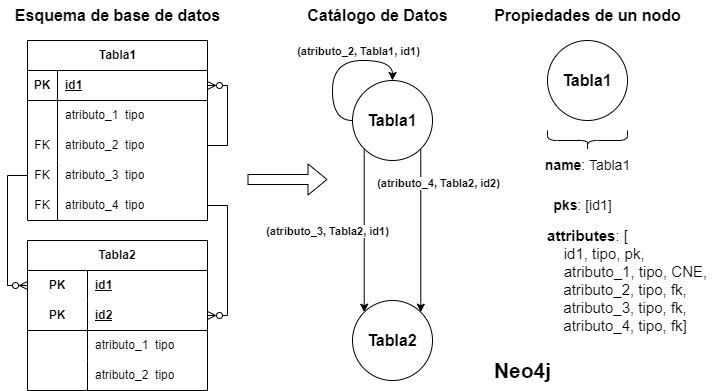
\includegraphics[width=0.7\textwidth]{Graphics/schema-catalog.drawio.png}
    \caption{Transición del esquema de bases de datos al cat\'alogo de datos}
    \label{fig:schema-catalog}
\end{figure}

La propiedad \textbf{attributes} en un nodo de un grafo del catálogo es una lista aplanada de los metadatos 
pues Neo4j no admite estructuras complejas 
como las listas de tuplas. Las siglas \textbf{CNE} significan \emph{constraint not specified} 
e indica que el atributo cuyo nombre se encuentra dos posiciones antes no es llave primaria o 
llave for\'anea. Cuando se construye el grafo de joins a partir del grafo del catálogo se retoma 
la estructura de lista de tuplas para la propiedad \textbf{attributes} como muestra la figura 
\ref{fig:catalog-jgraph}

\begin{figure}[H]
    \centering
    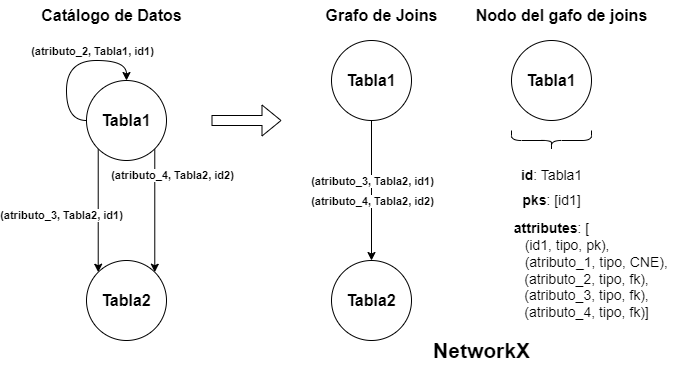
\includegraphics[width=0.7\textwidth]{Graphics/catalog-jgraph.drawio.png}
    \caption{Transición del catálogo de datos al grafo de joins}
    \label{fig:catalog-jgraph}
\end{figure}

\subsection{Generador de Consultas}

La implementación concebida para el generador de consultas est\'a compuesta por las implementaciones para el tratamiento de los scripts del lenguaje de 
dominio específico y generación de consultas, y por las implementaciones referentes a la construcci\'on 
y consulta de los \'arboles de join para la inferencia de joins.



\subsubsection{Lenguaje de Dominio Espec\'ifico}

La lógica del DSL se encuentra en la ruta \textbf{query\_generator/dsl}. El uso de la biblioteca 
PLY demanda la creación de dos scripts, uno donde se especifiquen los terminales de la gramática y las reglas 
para el análisis léxico y, otro, donde se especifiquen las producciones de la gramática mediante funciones. Estos 
scripts son \textbf{lexer.py} y \textbf{parser\_rules.py} respectivamente. En el script \textbf{ast\_nodes.py} se define  
la jerarquía de clases de los nodos del \'arbol de sintaxis abstracta (AST) del lenguaje de dominio específico expuesto 
en el capítulo \ref{chapter:proposal} y cuya gramática libre del contexto puede encontrarse en el ejemplo de 
c\'odigo \ref{code:CFG}. Cada 
estructura gramatical del lenguaje est\'a representada por una clase, como se muestra en la figura \ref{fig:ast}.

\begin{figure}[htb]
    \centering
    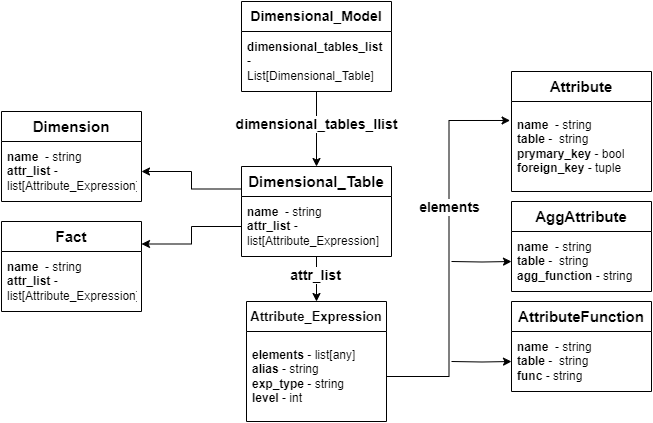
\includegraphics[width=0.7\textwidth]{Graphics/ast.png}
    \caption{Estructura del AST}
    \label{fig:ast}
\end{figure}

La clase \textbf{Dimensional\_Schema} representa un esquema dimensional en forma de estrella, el cual est\'a formado por una lista de tablas 
dimensionales \textbf{Dimensional\_Table}. Las clases \textbf{Dimension} y \textbf{Fact} heredan de \textbf{Dimensional\_Table} 
y representan a las dimensiones y a las tablas de hechos respectivamente. La clase \textbf{Attribute\_Expression} expresa 
la definición de un atributo, ya sea simple o una expresión aritmética donde participen varios atributos y n\'umeros. 
Las clases \textbf{Attribute}, \textbf{AggAttribute} y \textbf{AttributeFunction} representan atributos simples, atributos 
agregados y atributos resultado de la aplicación de alguna función respectivamente. El campo \textbf{foreign\_key} de 
la clase \textbf{Attribute}, en caso de tener alg\'un valor almacenado, es una tupla que indica que la instancia 
de \textbf{Attribute} es una llave for\'anea y en la primera posición de la tupla se almacena el nombre de la tabla referenciada y 
en la segunda posición, el nombre del atributo referenciado.

Una instancia de \textbf{Dimensional\_Schema} contiene una lista de instancias de \textbf{Dimensional\_Table}, las que a su vez pueden ser de tipo 
\textbf{Dimension} o \textbf{Fact}. Las instancias de \textbf{Dimension} o \textbf{Fact} poseen una lista de instancias de \textbf{Attribute\_Expression}, cada 
una de ellas presenta 
una lista llamada \textbf{elements} que puede contener uno o varios elementos; en caso de tener uno solo, el elemento 
es una instancia de \textbf{Attribute}, \textbf{AggAttribute} o \textbf{AttributeFunction}. En caso de tener 
m\'as de un elemento, es decir, la instancia de \textbf{Attribute\_Expression} representa un atributo compuesto, entonces 
\textbf{elements} contiene tanto las instancias de \textbf{Attribute}, \textbf{AggAttribute} o \textbf{AttributeFunction} como 
los signos de agrupación y operadores que participan en la definición del atributo.

Los scripts del DSL son tokenizados con la instancia de lexer declarada en \textbf{lexer.py}. La lista de tokens 
resultante pasa a ser analizada por la instancia de parser declarada en \textbf{parser\_rules.py}. El resultado 
del análisis sintáctico del parser es el \'arbol de sintaxis abstracta del script del DSL analizado.


\subsubsection{Generaci\'on de c\'odigo}

Luego de tener construido el árbol de sintaxis abstracta, AST, del script específico se pasa a realizar un análisis sobre 
esta estructura con 
el objetivo de detectar errores semánticos en el código del script. Si no se encuentran errores, 
a partir del AST se comienza a generar el código de las consultas de creación y selección.

Siguiendo las mejores prácticas de la industria, todos los análisis sobre el AST se realizan 
utilizando el patrón visitor\cite{buttner2004digging}. Cada nodo del AST implementa la clase abstracta 
\textbf{Visitable} presente en \textbf{visitable.py}. El ejemplo de c\'odigo \ref{code:visitable} 
muestra el c\'odigo de la clase \textbf{Visitable}.

\begin{lstlisting}[label={code:visitable}, caption={Clase abstracta Visitable}, language={python}]
    import abc

    class Visitable(metaclass = abc.ABCMeta):
        @abc.abstractmethod
        def accept(self, visitor):
            pass
\end{lstlisting}

Por tanto, todo nodo del AST posee un método \textbf{accept} que recibe un visitor específico. La implementación 
puntual de \textbf{accept} para cada tipo de nodo del AST consiste en llamar al método \textbf{visit}, del visitor pasado como argumento, 
que le corresponde a su tipo. Los visitors implementados pueden encontrarse en el script \textbf{visitors.py} y la 
figura \ref{fig:visitors} muestra la jerarquía de clases de los visitors implementados.

\begin{figure}[htb]
    \centering
    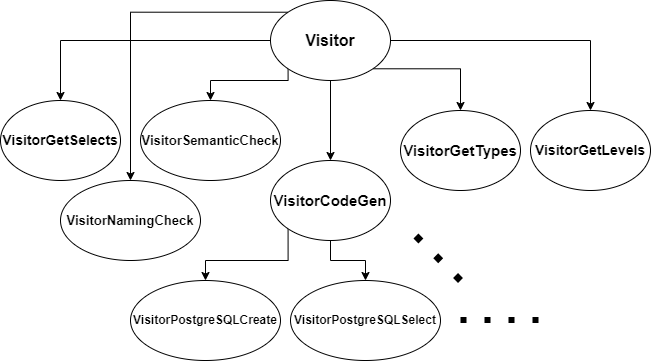
\includegraphics[width=0.7\textwidth]{Graphics/visitorfixed.drawio.png}
    \caption{Jerarquía de Visitors}
    \label{fig:visitors}
\end{figure}

La clase \textbf{Visitor} es la raíz de la jerarquía. Es una clase abstracta en la que se definen los métodos 
\textbf{visit} que deben tener todas las clases herederas. En particular, hay un \textbf{visit} por cada tipo de 
nodo del AST, lo que se detalla en el ejemplo de c\'odigo \ref{code:visitors}

\begin{lstlisting}[label={code:visitors}, caption={Clase Visitor}, language={python}]
    class Visitor(metaclass = abc.ABCMeta):
        @abc.abstractmethod
        def visit_dimensional_schema(self, dimensional_model): pass 

        @abc.abstractmethod
        def visit_attribute(self, attribute): pass

        @abc.abstractmethod
        def visit_attr_function(self, attr_func): pass

        @abc.abstractmethod
        def visit_agg_attr(self, agg_attr): pass

        @abc.abstractmethod
        def visit_attr_expression(self, attr_expression): pass

        @abc.abstractmethod
        def visit_dimensional_table(self, dimensional_table): pass
\end{lstlisting}

Las instancias de las clases \textbf{VisitorSemanticCheck}, \textbf{VisitorNamingCheck}, \textbf{VisitorGetTypes} 
son las encargadas de realizar
controles semánticos sobre el código del script del DSL analizado. Las instancias de \textbf{VisitorSemanticCheck} realizan los siguientes 
chequeos:

\begin{itemize}
    \item Revisan si en el esquema estrella definido existe al menos una dimensión y una tabla de hechos.
    \item Se aseguran que las tablas definidas tengan al menos un atributo válido.
    \item Se aseguran que todas las tablas tengan definidas al menos una llave primaria.
    \item Verifican que no existan llaves for\'aneas declaradas en atributos compuestos.
    \item Verifican que tanto los atributos referenciados como las tablas referenciadas est\'en definidos en el 
        script.
    \item Revisan si las tablas y los atributos fuente utilizados en el script existen en la base de datos fuente.
    \item Verifican el correcto uso de la palabra reservada \textbf{self}.
\end{itemize}

Las instancias de \textbf{VisitorNamingCheck} se encargan de recorrer el AST y verificar que: 

\begin{itemize}
    \item En las dimensiones o tablas de hechos no existan dos atributos definidos con el mismo nombre.
    \item No existan dos tablas del esquema estrella con el mismo nombre.
    \item Los atributos compuestos definidos tengan asignados un alias para su correcta identificación.
\end{itemize}

Las instancias de \textbf{VisitorGetTypes} son las responsables de verificar el buen uso de los tipos en el 
código del DSL además de recolectar el tipo de cada atributo declarado en cada dimensión y 
en la tabla de hechos, 
información necesaria para el proceso de generación de código. En particular, realizan 
las siguientes verificaciones: 

\begin{itemize}
    \item Verifican que los atributos compuestos definidos se les haya especificado su tipo.
    \item En el caso de las llaves for\'aneas comprueban que la llave for\'anea y el atributo referenciado 
        coincidan en tipo.
\end{itemize}

Las instancias de \textbf{VisitorGetSelects} se encargan de recorrer el AST y por cada tabla dimensión o tabla 
de hechos recolectan las tablas y los atributos que hay que seleccionar de la fuente de datos 
para poblar las tablas respectivas. A partir de esta información se confeccionan las consultas 
que se realizan a los \'arboles de join para obtener el join necesario para el proceso de población.

Las instancias de \textbf{VisitorGetLevel} son las encargadas de recopilar los niveles de cada uno de los 
atributos de las tablas del esquema estrella. Esta información luego se exportar\'a al almacén de datos 
destino en forma de una tabla de metadatos llamada \textbf{level\_metadata}. Dicha tabla tendrá tres atributos: 
\textbf{table\_name}, \textbf{attribute\_name} y \textbf{level}. El primero es el nombre de la tabla del esquema 
estrella, el segundo es el nombre del atributo y el tercero es un entero que representa el nivel del atributo 
en la jerarquía de la tabla con nombre \textbf{table\_name}.

La clase \textbf{VisitorCodeGen} es una clase abstracta de la que heredar\'an todos los visitors que 
se encarguen de generar código. Hereda de la clase \textbf{Visitor} y la extiende pues incorpora un 
método para exportar las consultas generadas, como se muestra en el ejemplo de c\'odigo \ref{code:vcodegen}.

\begin{lstlisting}[label={code:vcodegen}, caption={Clase VisitorCodeGen}, language={python}]
    class VisitorCodeGen(Visitor):
        def visit_dimensional_model(self, dimensional_model):
            return super().visit_dimensional_model(dimensional_model)
        def visit_dimensional_table(self, dimensional_table):
            return super().visit_dimensional_table(dimensional_table)
        def visit_attr_expression(self, attr_expression):
            return super().visit_attr_expression(attr_expression)
        def visit_attribute(self, attribute):
            return super().visit_attribute(attribute)
        def visit_attr_function(self, attr_func):
            return super().visit_attr_function(attr_func)
        def visit_agg_attr(self, agg_attr):
            return super().visit_agg_attr(agg_attr)

        @abc.abstractmethod
        def export_querys(self): pass
\end{lstlisting}

La generación de código es otro de los puntos de dependencia del prototipo con los sistemas de gestión 
de bases de datos. Específicamente, las consultas de selección dependen del sistema de gestión de bases 
de datos de la fuente, pues estas se encargan de extraer los datos para la población, y las consultas 
de creación dependen del sistema de gestión de bases de datos del almacén de datos de destino, pues 
son las responsables de crear las tablas del esquema estrella. Para resolver esta dependencia 
se implementa un visitor para la generación de las consultas de selección y un visitor para la generación 
de las consultas de creación, por cada sistema de gestión de bases de datos, como se muestra en la 
figura \ref{fig:visitors}. De esta forma, cada tipo de consulta la genera el visitor que le corresponde 
al sistema de gestión de bases de datos de la fuente o del destino. En esta primera versión del prototipo 
se implementaron los visitors de generación de código para PostgreSQL.

Las instancias de la clase \textbf{VisitorPostgreSQLCreate} son las encargadas de generar las 
consultas de creación de las tablas del esquema estrella para el sistema gestor PostgreSQL. En la 
declaración de los atributos 
dentro de la consulta se utiliza la información recolectada por \textbf{VisitorGetTypes} para 
especificar los tipos de los atributos que se crear\'an. Pero las instancias de \textbf{VisitorGetTypes} 
recolectan los tipos que maneja el DSL, por tanto, cada instancia de \textbf{VisitorPostgreSQLCreate} 
tiene un diccionario que mapea los tipos del DSL a los tipos de PostgreSQL.

Las instancias de la clase \textbf{VisitorPostgreSQLSelect} generan las consultas de selección para 
el sistema gestor PostgreSQL. Reciben los joins seleccionados por el desarrollador para cada tabla del esquema 
estrella y conforman las consultas de selección.

\subsubsection{Inferencia de joins}

La implemetaci\'on de la l\'ogica para la inferencia de joins se encuentra repartida 
en los scripts de Python \textbf{maximal\_join\_trees.py}, \textbf{join\_computation.py} y 
\textbf{all\_spanning\_trees.py}. 

A modo de recordatorio, en el cap\'itulo de concepción y diseño se expuso que los \'arboles de expansión 
de los grafos alcanzables originados desde nodos del grafo de join con indegree cero, o pertenecientes 
a una componente fuertemente conexa sin arcos incidentes exteriores, constituyen el conjunto de \'arboles 
de join a partir de los cuales se realizar\'a la inferencia de joins.

En script \textbf{all\_spanning\_trees.py} yacen los algoritmos para la obtención de los \'arboles de expansión 
de un grafo alcanzable, como se muestra en el ejemplo de c\'odigo \ref{code:stgen}.

\begin{lstlisting}[label={code:stgen}, caption={Algoritmo para la generación de \'arboles de expansión}, language={python}]
    def networkX_all_spanning_trees(graph:DiGraph) -> list[DiGraph]:
        result = []
        for tree in ArborescenceIterator(graph):
            result.append(tree)

        return result
\end{lstlisting}

En esta primera entrega solo se implement\'o una variante que se apoya en la 
clase ArborescenceIterator de NetworkX, la cual constituye un iterador de los \'arboles de expansión de un digrafo 
pasado como argumento.


En el script \textbf{maximal\_join\_trees.py} yace
la implementación en Python del pseudoc\'odigo propuesto para la fase de precomputaci\'on, en el 
capítulo \ref{chapter:proposal} en la sección del generador de consultas, específicamente en el ac\'apite referido 
a la inferencia de joins, ver ejemplo de c\'odigo \ref{precom}. El m\'etodo \textbf{maximal\_join\_trees\_generator} 
constituye la implementación del pseudoc\'odigo de la fase de precomputaci\'on y toma como argumentos 
un grafo de joins y devuelve una lista de \'arboles de join. Los \'arboles de join también son digrafos de 
NetworkX con las mismas propiedades definidas para los nodos y arcos que presenta el grafo de joins, 
ilustradas en la figura \ref{fig:catalog-jgraph}.

Para la generación de los \'arboles de join, \textbf{maximal\_join\_trees\_generator} se apoya en 
el m\'etodo \textbf{\_find\_reachable} para calcular el grafo alcanzable desde un nodo ra\'iz en el grafo 
de joins y del m\'etodo \textbf{\_in\_edge\_from\_outside} para verificar si una componente fuertemente 
conexa posee arcos incidentes desde el exterior. Las componentes fuertemente conexas son calculadas 
utilizando el m\'etodo \textbf{strongly\_connected\_components} de la biblioteca NetworkX. A los nodos 
de los \'arboles generados se les añade, mediante el método \textbf{\_set\_height}, la propiedad \textbf{height} que almacena 
la altura del nodo con respecto a la raíz del \'arbol, con el objetivo de facilitar el c\'omputo 
del ancestro com\'un m\'as bajo de un conjunto de nodos. Por \'ultimo, 
los árboles de join son almacenados en la ruta \textbf{data/join\_trees}.


El script \textbf{join\_computation.py} alberga el m\'etodo \textbf{compute\_joins}, el cual es la implementación 
en Python del algoritmo \textbf{get\_joins} cuyo pseudoc\'odigo fue expuesto en el capítulo \ref{chapter:proposal} 
en el ejemplo de c\'odigo \ref{querytime}. El ejemplo de c\'odigo \ref{computejoins} muestra el c\'odigo del 
m\'etodo \textbf{compute\_joins}.

\begin{lstlisting}[label={computejoins}, caption={C\'odigo del m\'etodo \textbf{compute\_joins}}, language={python}]
    def compute_joins(join_trees: list[DiGraph], tables_list) -> str:
        valid_join_trees = _get_answer_trees(join_trees, tables_list)
        all_joins = []
        for tree in valid_join_trees:
            lca = _lowest_common_ancestor(tree, tables_list)
            join = _get_join(tree, lca, tables_list)
            if join not in all_joins:
                all_joins.append(join)

        return all_joins
\end{lstlisting}

Este algoritmo recibe la lista de \'arboles de joins generados y una 
lista de tablas a concatenar y devuelve una lista de joins. La lista de tablas a concatenar es provista por el 
visitor \textbf{VisitorGetSelects}. El m\'etodo \textbf{\_get\_answer\_trees} dado una lista de 
\'arboles de join y una lista de tablas a concatenar devuelve los \'arboles de join que contienen todas las tablas de 
la consulta, representada en la lista \textbf{tables\_list}, y por tanto pueden proporcionar interpretaciones 
para la consulta. El m\'etodo \textbf{\_lowest\_common\_acestor} calcula el ancestro com\'un m\'as bajo, LCA, para el 
conjunto de tablas en \textbf{tables\_list}. El m\'etodo \textbf{\_get\_join} construye el subárbol del \'arbol 
de join \textbf{tree}, que constituye una interpretaci\'on de la consulta para dicho \'arbol de join, y lo 
convierte en una lista que representa una secuencia de joins para facilitar el proceso de generación del c\'odigo del join computado. 
Los componentes de la lista que representa una secuencia de joins se alternan entre el nombre de las tablas 
y una lista con tuplas que representan las condiciones del join entre las tablas. El ejemplo de c\'odigo \ref{joinlist}
ilustra la estructura de la lista que representa una secuencia de joins.

\begin{lstlisting}[label={joinlist}, caption={Estructura de una lista que representa una secuencia de joins}, language=python]
    ['tabla1', [('tabla1.atr1', 'tabla2.atr2'), ...], 'tabla2', ...]
\end{lstlisting}

La lista del ejemplo de c\'odigo \ref{joinlist} representa el join entre las tablas \textbf{tabla1} y \textbf{tabla2} 
bajo la condición (\textbf{tabla1.atr1 = tabla2.atr2 and ...}). Por supuesto, la secuencia de joins 
que representa una lista con esta estructura no est\'a limitada a un join entre solo dos tablas.

N\'otese que como los \'arboles de join comparten las propiedades del grafo de joins, mediante un recorrido 
DFS sobre el subárbol que representa una interpretaci\'on de una consulta sobre un \'arbol de join determinado, se puede 
obtener una lista con la estructura que se muestra en el ejemplo de c\'odigo \ref{joinlist}. 

La figura \ref{fig:allpro} muestra como interactúan los componentes anteriormente explicados 
para obtener, a partir de la definición de un escenario anal\'itico, las consultas de creación y las consultas de  
selección.

\begin{figure}[H]
    \centering
    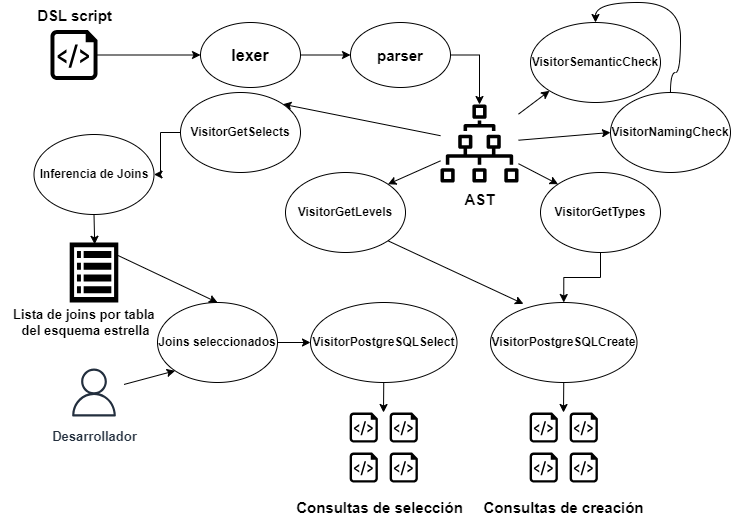
\includegraphics[width=0.7\textwidth]{Graphics/all_procces.drawio.png}
    \caption{Proceso de generación de consultas desde el inicio.}
    \label{fig:allpro}
\end{figure}

\subsection{Interfaz de Usuario}

Para la implementación de la interfaz de usuario se utilizó la biblioteca Streamlit de Python. Esta biblioteca 
permite la implementación de aplicaciones web mediante la definición de scripts de Python donde se 
definan los componentes de las páginas de la aplicación mediante la API de Streamlit. Además, proporciona un 
servidor para alojar la aplicación e interactuar con ella. La interfaz de usuario de la aplicación cuenta 
con cuatro páginas. La página principal se define en el directorio raíz de la aplicación y el resto de las 
páginas dentro de una carpeta llamada \textbf{pages}. 

\subsubsection{Main Page}

Esta es la página principal de la aplicación, cuya imagen se muestra en la figura \ref{fig:mainpage} como anexo. 
En el script \textbf{Main\_Page.py} se definen 
los componentes de la página. En Main Page el desarrollador deber\'a establecer la conexión con un servidor de 
bases de datos fuente y escoger si desea realizar un proceso de recomputaci\'on de la conexión. El 
proceso de recomputaci\'on consiste en crear una instancia de crawler para explorar la base de datos 
fuente, crear la base de datos de Neo4j correspondiente al esquema de la fuente de datos en el catálogo 
de datos y exportar el grafo de join y los \'arboles de join derivados. Como se expuso en el capítulo 
\ref{chapter:proposal} este cómputo es costoso, por tanto solo est\'a pensado para realizarse la primera 
vez que se descubre la base de datos fuente o cuando el esquema de la misma sufra cambios. En este \'ultimo caso, 
el catálogo de datos, el grafo de join y los \'arboles de join serían inválidos y necesitan ser recalculados. 
Además, la página cuenta con un formulario para registrar nuevos servidores de bases de datos. La información 
de los servidores es almacenada en la ruta \textbf{data/connections} en formato json.

\subsubsection{Metadata}

En esta página se muestran los metadatos recopilados por el crawler, as\'i como las imágenes del 
grafo de join y los \'arboles de join derivados. El script de esta página es \textbf{Metadata.py} y 
la imagen se muestra en la figura \ref{fig:meta} como anexo.

\subsubsection{Query Generator}

En esta página se muestran las consultas generadas. Como anexos se incluyen la imagen de la página 
Query Generator en la figura \ref{fig:generator}, así como fragmentos de consultas generadas en 
la figura \ref{fig:qfragment}.
Primero se selecciona un script del DSL que 
define un esquema estrella a poblar. Luego se debe escoger, por cada tabla del esquema estrella, el 
join que mejor se ajuste para la extracción de los valores. La selección se realiza a través 
de componentes en la interfaz de usuario. Una vez seleccionados los joins, aparecer\'a un bot\'on 
para comenzar el proceso de generación de las consultas  
de creación y de selección para cada tabla del esquema estrella, as\'i como la consulta 
para crear y poblar la tabla de metadatos \textbf{level\_metadata}. Las consultas generadas 
son almacenadas en la ruta \textbf{data/querys}, lo que posibilita su recuperación y descarga por parte del desarrollador. 
Todo el proceso de generación y análisis del script del DSL es mediado por la clase \textbf{Orchestrator}, 
presente en \textbf{orchestrator.py}, como se muestra en el ejemplo de c\'odigo \ref{code:orchestrator}.

\begin{lstlisting}[label={code:orchestrator}, caption={Clase Orchestrator}, language={python}]
    class Orchestrator:
        def __init__(self, dbname, dwname, source_sgbd, target_sgbd, script) -> None:
            # Omitted Implementation

        def parse_code(self, code):
            # Omitted Implementation

        def compute_joins(self):
            # Omitted Implementation

        def generate_querys(self, selected_joins):
            # Omitted Implementation
\end{lstlisting}

Los campos de la clase son \textbf{dbname} que es el nombre de la base de datos fuente, 
\textbf{dwname} que es el nombre del almacén de datos de destino, \textbf{source\_sgbd} y 
\textbf{target\_sgbd} que son respectivamente los sistemas gestores de bases de datos de la fuente de datos y 
del almacén de datos de destino, y \textbf{script} que es una cadena de texto con el código 
de definición del esquema estrella a poblar.

El método \textbf{parse\_code} se encarga de tomar el código en \textbf{script}, parsearlo 
con la instancia de parser de \textbf{PLY} para obtener el árbol de sintaxis abstracta AST correspondiente. 
Luego dicho AST se somete a los recorridos de todos los visitors requeridos para la detección de errores semánticos. Si se 
encuentran anomalías en el código, se añaden los mensajes respectivos al archivo \textbf{dsl\_log.log} 
que se mostrarán al desarrollador convenientemente. Si no se detectan anomalías, entonces se pasa a computar los joins. 

El método \textbf{compute\_joins} recupera los \'arboles de joins almacenados para la base de datos 
fuente en cuestión. A partir de la información recopilada por la instancia de visitor \textbf{VisitorGetSelect}, 
por cada tabla del esquema estrella se computa un conjunto de posibles joins para conformar la consulta 
de selección, utilizando el algoritmo de inferencia de joins expuesto en el ejemplo de código \ref{querytime}. 
Despu\'es de este proceso, el desarrollador debe seleccionar 
los joins de su conveniencia para la conformación de las consultas de selección. 

Por \'ultimo, el método \textbf{generate\_querys} se encarga de tomar los joins, seleccionados por el desarrollador para 
cada tabla del esquema estrella, y conformar las consultas de creación y de selección. Los visitors 
correspondiente para la generación de ambas consultas se seleccionan utilizando los campos 
\textbf{source\_sgbd} y \textbf{target\_sgbd}. Las consultas generadas son mostradas en la interfaz y pueden ser descargadas 
por el desarrollador para construir manualmente un pipeline válido. 
Las consultas son descargadas en archivos separados con extensión .sql.

\subsubsection{Logs}

En esta página se muestran los errores en la definición del esquema
estrella encontrados por los visitors, así como información de interés
respecto a la ejecución de la aplicación. En la figura \ref{fig:logs} se muestra una imagen de la 
página como anexo.